\documentclass{beamer}

\usepackage[czech]{babel}
\usepackage[utf8]{inputenc}
\usepackage[normalem]{ulem}
\usepackage{mathtools}
\usepackage{amssymb}
\usepackage{pifont}
\usepackage{color}
\usepackage{multirow}
\newcommand{\cmark}{\ding{51}}%
\newcommand{\xmark}{}%

\usetheme{Madrid}
%\usecolortheme{beaver}

\newcommand{\metric}[1]{\textsc{#1}}
\newcommand{\baseline}[1]{\textcolor{blue}{\textsc{#1}}}

\newcommand{\XXX}[1]{\textcolor{red}{XXX #1}}

%\definecolor{barva1}{HTML}{071988}
%\definecolor{barva2}{HTML}{202F87}
%\definecolor{barva3}{HTML}{3A4587}
%\definecolor{barva4}{HTML}{535B87}
%\definecolor{barva5}{HTML}{6D7187}
%\definecolor{barva6}{HTML}{878787}

\definecolor{barva1}{HTML}{e60000}
\definecolor{barva2}{HTML}{e63408}
\definecolor{barva3}{HTML}{e6650F}
\definecolor{barva4}{HTML}{e69317}
\definecolor{barva5}{HTML}{e6be1F}
\definecolor{barva6}{HTML}{e6e626}

\newcommand{\best}[1]{\textbf{#1}}

\newcommand{\rangeA}[1]{\textcolor{barva1}{#1}}
\newcommand{\rangeB}[1]{\textcolor{barva2}{#1}}
\newcommand{\rangeC}[1]{\textcolor{barva3}{#1}}
\newcommand{\rangeD}[1]{\textcolor{barva4}{#1}}
\newcommand{\rangeE}[1]{\textcolor{barva5}{#1}}
\newcommand{\rangeF}[1]{\textcolor{barva6}{#1}}

\def\oosmark#1{\llap{$\wr$\, }#1}  % out-of-sequence mark
\def\pojem#1{\textit{#1}}  % definice terminu

\newenvironment<>{cvarblock}[2][\textwidth]{
    \begin{center}
      \begin{minipage}{#1}
        \setlength{\textwidth}{#1}
          \begin{actionenv}#3
            \def\insertblocktitle{#2}
            \par
            \usebeamertemplate{block begin}}
  {\par
      \usebeamertemplate{block end}
    \end{actionenv}
  \end{minipage}
\end{center}}

\beamertemplatenavigationsymbolsempty

\title{Měření kvality strojového překladu}
\subtitle{Diplomová práce}
\author{Matouš Macháček}
\institute[UK]{Univerzita Karlova v Praze}
\date{2014}
% \pgfdeclareimage[height=0.5cm]{university-logo}{university-logo-filename}
% \logo{\pgfuseimage{university-logo}}

\begin{document}

\begin{frame}
  \titlepage
\end{frame}

\begin{frame}{Evaluace strojového překladu}
    \begin{itemize}
        \item Podobně jako u jiných úloh je evaluace velmi důležitá
        \begin{itemize}
            \item Při vývoji systému je potřeba měřit zlepšní
        \end{itemize}
        \pause
        \vspace{0.5em}
        \item Na rozdíl od jiných úloh je evaluace strojového překladu velmi obtížná
        \begin{itemize}
            \item Neexistuje jeden jediný správný výstup
        \end{itemize}
        \pause
        \vspace{0.5em}
        \item Dva základní přístupy
        \begin{itemize}
            \item \textbf{Manuální evaluace} - Lidé hodnotí kvalitu přeložených vět ručně
            \item \textbf{Automatická evaluace} - Automatická metrika měří podobnost
                s~referenčním překladem

        \end{itemize}
        
    \end{itemize}
\end{frame}

\begin{frame}{Cíle diplomové práce}
    \begin{itemize}
        \item V diplomové práci zkoumám oba přístupy
        \vspace{0.5em}
        \pause
    \item \textbf{Manuální evaluace}
        \begin{enumerate}
            \item Navrhnout novou manuální evaluační metodu,
            \begin{itemize}
                \item která bude jednodušší a rychlejší pro anotátory a spolehlivější
            \end{itemize}
            \item Navrhnout uživatelský přívětivé anotační prostředí
            \item Provést evaluační experiment
            \item Použít získanou databázi anotací pro evaluaci nových, neviděných překladů
        \end{enumerate}
        \vspace{0.5em}
        \pause
    \item \textbf{Automatická evaluace}
        \begin{enumerate}
            \item Porovnat zkoumané metriky kvalitativně i kvantitativně
            \begin{itemize}
                \item Využil jsem možnosti organizovat soutěž strojových metrik na WMT
            \end{itemize}
        \end{enumerate}
    \end{itemize}
\end{frame}

\begin{frame}{Stávající evaluační metoda používaná na WMT}
    \begin{itemize}
        \item Anotátoři porovnávají celé věty relativně vůči sobě
        \item Pro dlouhé věty to bývá náročné a pomalé
    \end{itemize}
    \begin{center}
        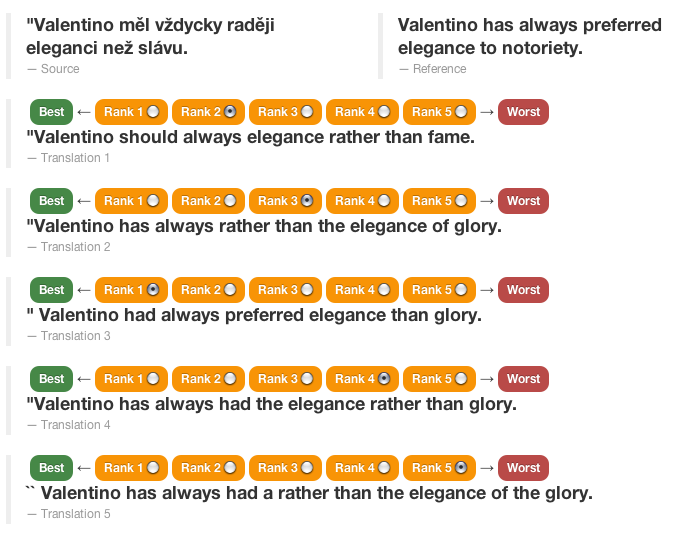
\includegraphics[width=6cm]{rankingtask.png}
    \end{center}
\end{frame}

    
\begin{frame}{SegRanks - Navrhovaná metoda}
    \begin{itemize}
        \item Věta je rozdělena na kratší segmenty (úseky)
    \pause
        \item Shodné segmenty vyprodukované různými systémy jsou sjednoceny
    \pause
        \item Anotátoři porovnávají pouze krátké segmenty
    \end{itemize}
    \pause
    \begin{center}
        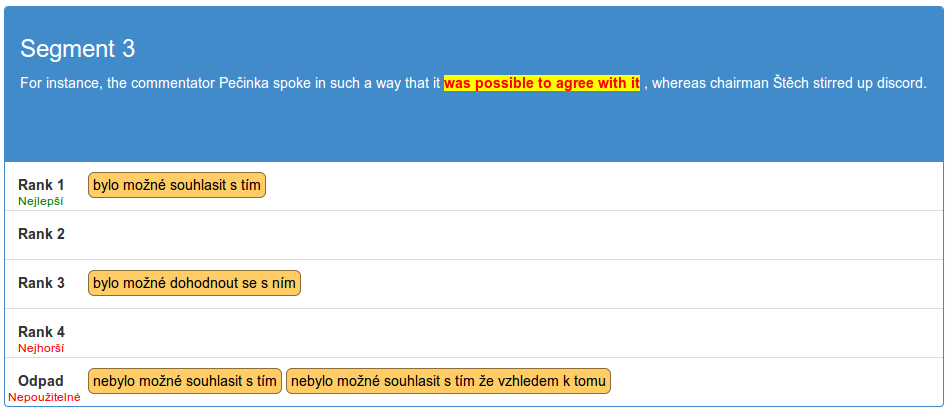
\includegraphics[width=10cm]{screenshot-small.png}
    \end{center}
\end{frame}

\begin{frame}{Extrakce segmentů}
    \begin{center}
        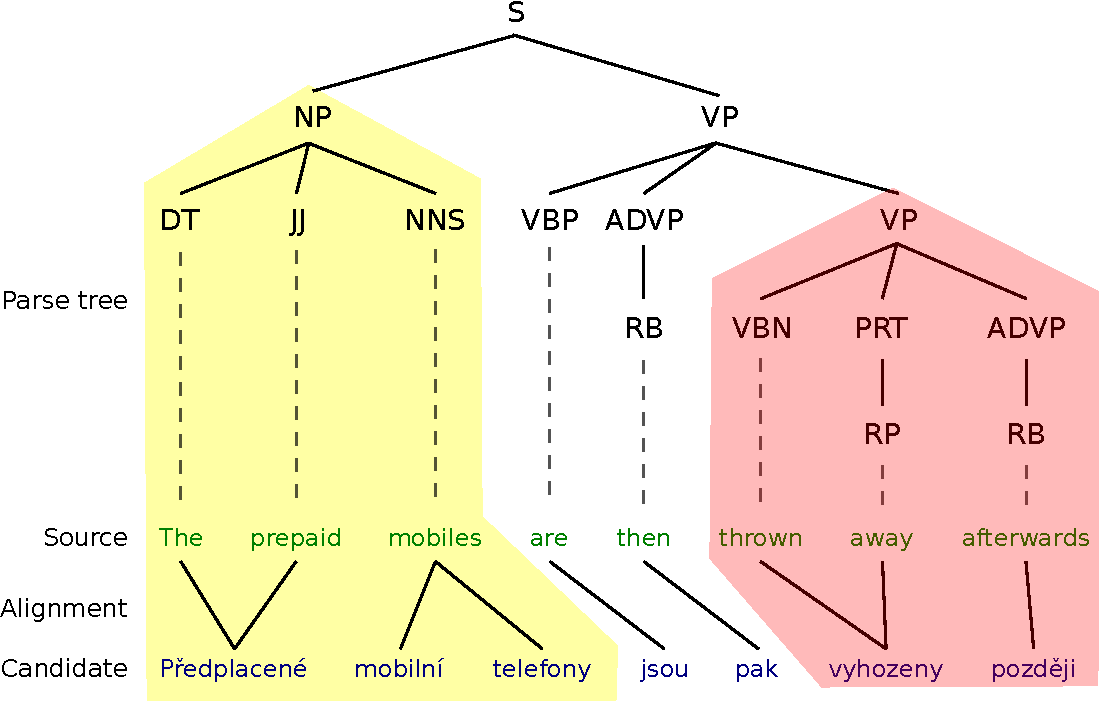
\includegraphics[width=10cm]{tree-align.pdf}
    \end{center}
\end{frame}

%\begin{frame}{Segranks annotation interface}
    %\begin{center}
        %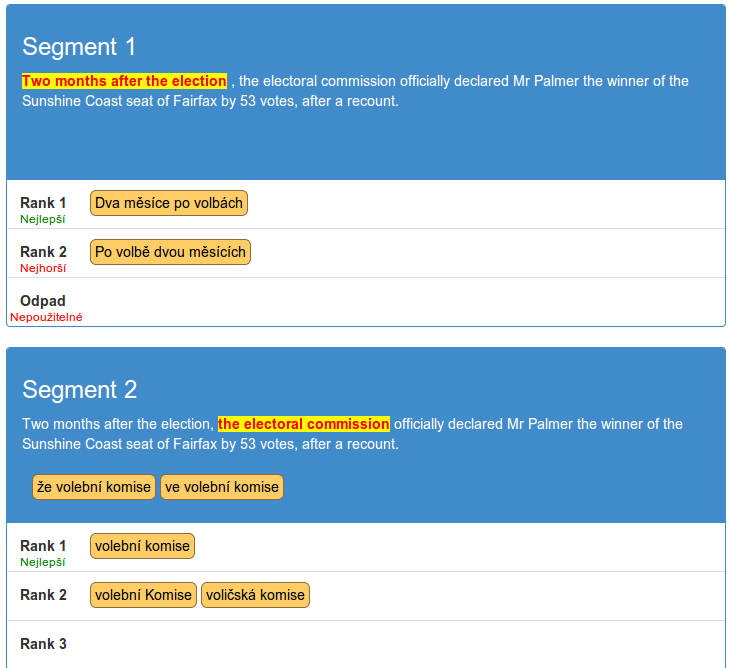
\includegraphics[width=8cm]{segranks-screenshot.png}
    %\end{center}
%\end{frame}

\begin{frame}{Provedené experimenty 1/4}
    \begin{itemize}
        \item Provedl jsem evaluační experiment na datech WMT ve směru do češtiny
    \pause
        \item Celkové hodnocení systémů získané novou metodou je velmi podobné oficiálnímu WMT hodnocení
    \pause
        \item Mezianotátorská shoda mírně lepší
    \end{itemize}
    \begin{cvarblock}[8cm]{Anotátorské shody}
    \begin{center}
        \begin{tabular}{r|cc}
            & WMT & SegRanks \\
            \hline
            intra-annotator $\kappa$ & 0.448 &  0.593      \\
            inter-annotator $\kappa$ & 0.360 &  0.397      \\
        \end{tabular}
    \end{center}
    \end{cvarblock}
\end{frame}

\begin{frame}{Provedené experimenty 2/4}
    \begin{itemize}
        \item Použití získané databáze pro evaluaci nových, neviděných překladů
    \pause
        \item Využívám toho, že 58.8 \% segmentů z neviděných překladů se nacházelo v databázi
    \pause
        \vspace{0.5em}
        \item Počítání skóre pouze na těchto segmentech však nefunguje
        \begin{itemize}
            \item Překladové systémy se častěji shodnou na kvalitnějších překladech, než na těch horších
            \item Nové, neviděné překlady jsou proto velmi nadhodnoceny
        \end{itemize}
    \end{itemize}
\end{frame}

\begin{frame}{Provedené experimenty 3/4}
    \begin{itemize}
    \pause
        \item Potřeba extrapolovat hodnocení i neviděných segmentů
    \pause
        \item Přirozené řešení je použít hodnocení nejbližšího segmentu, který je v databázi (KNN pro $k=1$)
    \pause
        \item Bohužel nefunguje, nejbližší segmenty mají většinou lepší hodnocení
    \end{itemize}
    \pause
    \begin{center}
        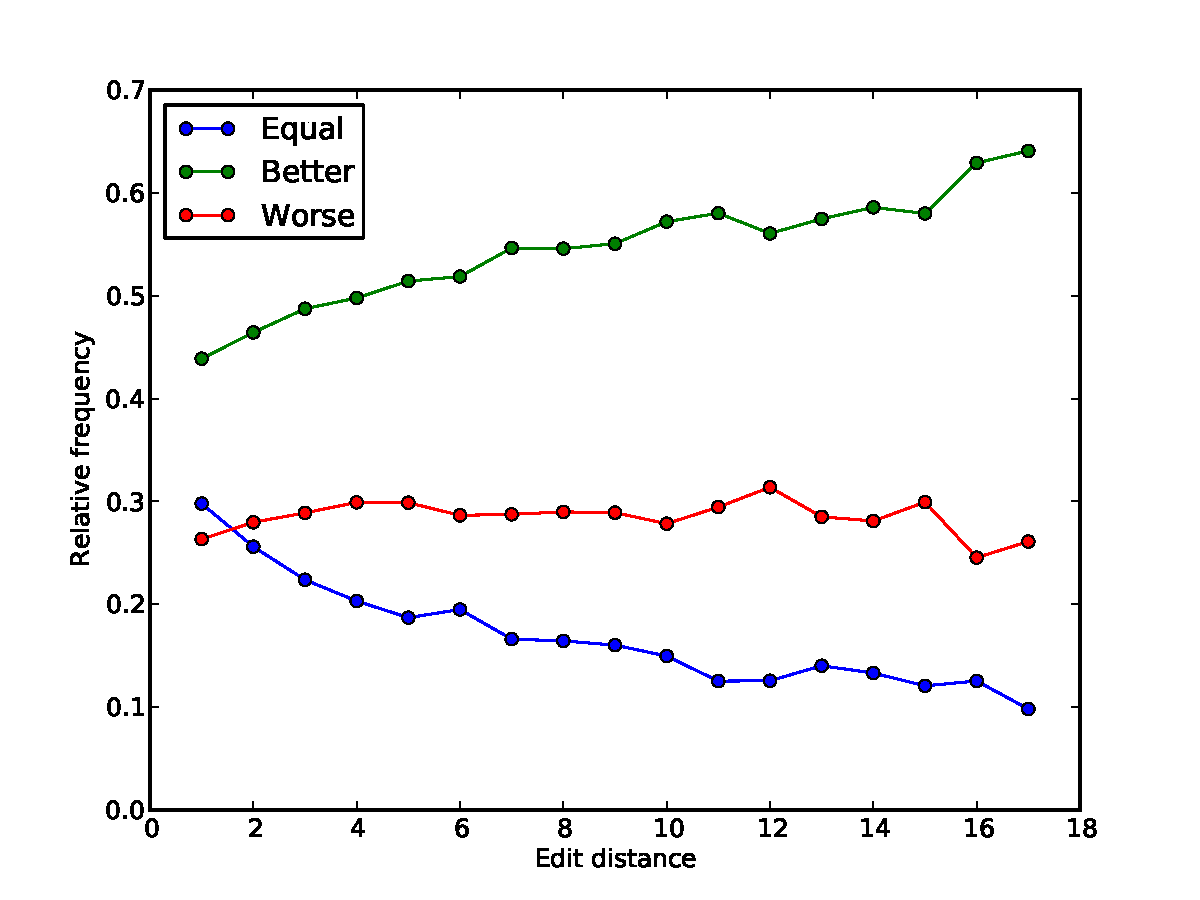
\includegraphics[width=8cm]{per-distance.pdf}
    \end{center}
\end{frame}

\begin{frame}{Provedené experimenty 4/4}
    \begin{itemize}
        \item Nakonec jsem použil databázi anotací pro ladění statistického strojového překladače
    \pause
        \item Metoda \textbf{MERT} nalezne optimální váhy loglineárního modelu
    \pause
        \item Vyzkoušel jsem několik variant
    \pause
        \item Vyladěné systémy jsem pak manuálně porovnal proti baseline
    \pause
    \end{itemize}
    \begin{cvarblock}{Výsledky}
        \begin{center}
  \begin{tabular}{r|c|cc}
    \textbf{Metrika použitá k ladění} & \textbf{iterace} & \textbf{Lepší} & \textbf{Horší} \\
    \hline
        %\metric{BLEU} (baseline) & 11 &  --- & --- \\
    \metric{ExactMatch}      & 20 &  22 \% & 38 \% \\
    \metric{PenalizeUnknown} &  8 & \textbf{34 \%} & \textbf{25 \%} \\
    \metric{SegRanksBLEU}    &  8 & 29 \% & 49 \% \\
  \end{tabular}
        \end{center}
    \end{cvarblock}
\end{frame}
    
\begin{frame}{Soutěž automatických metrik v kostce}
    \vspace{-0.5em}
    \begin{center}
    \includegraphics<2>[width=10cm]{metrics-task-diagram-1.png}
    \includegraphics<3>[width=10cm]{metrics-task-diagram-2.png}
    \includegraphics<4>[width=10cm]{metrics-task-diagram-3.png}
    \includegraphics<5>[width=10cm]{metrics-task-diagram-4.png}
    \includegraphics<6>[width=10cm]{metrics-task-diagram-5.png}
    \includegraphics<7>[width=10cm]{metrics-task-diagram-6.png}
%    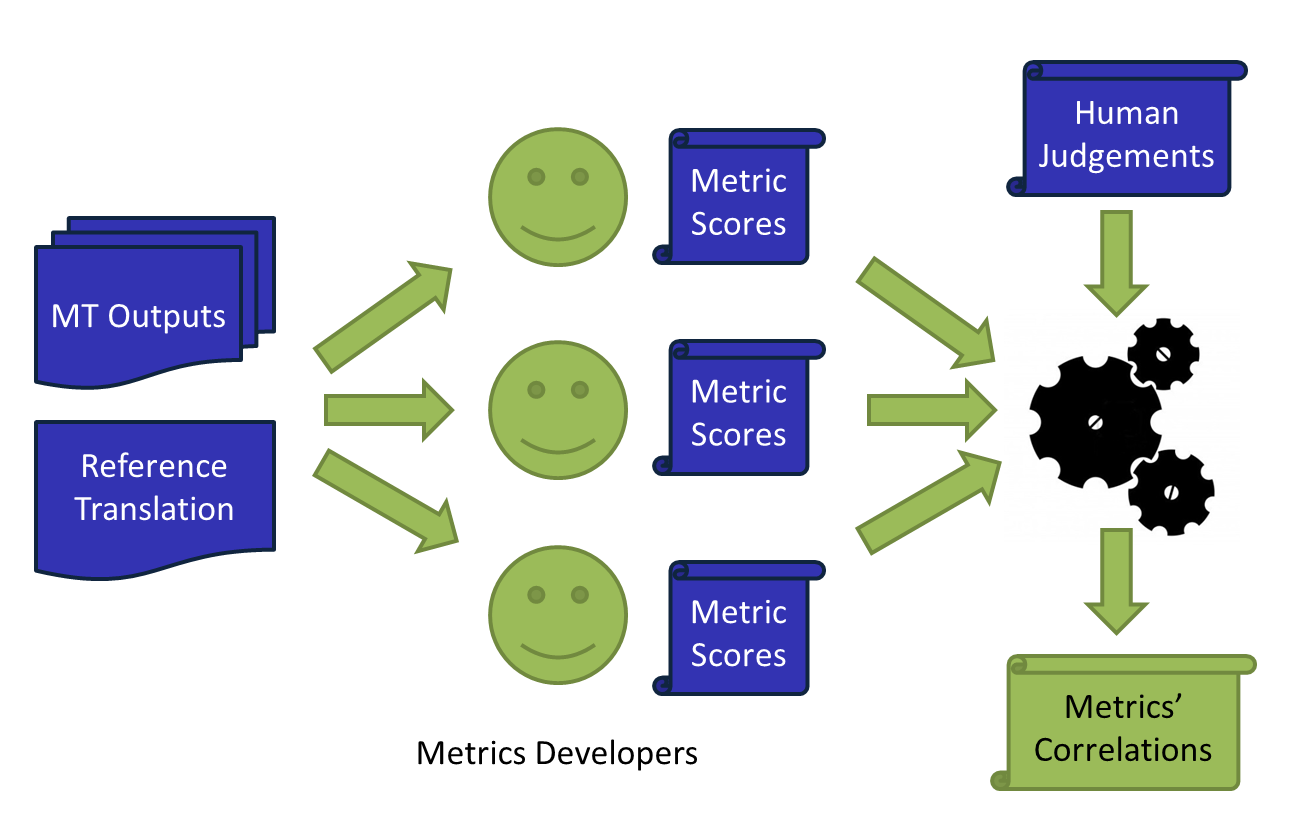
\includegraphics[width=10cm]{metrics-task-diagram-6.png}
   \end{center}
\end{frame}

%\begin{frame}{Dvě podúlohy}
%    \pause
%    \begin{columns}[T]
%        \begin{column}{7cm}
%          \begin{itemize}
%              \item \textbf{Úrověn systémů}
%            \begin{itemize}
%              \item Metrika vyprodukovala jedno skóre pro celý přeložený dokument
%              %\item Pro každou metriku jsem vypočítal korelaci mezi metrikou a
%              %    oficiálním lidským skórem
%            \end{itemize}
%          \end{itemize}
%      \end{column}
%      \begin{column}{3cm}
%          \begin{center}
%            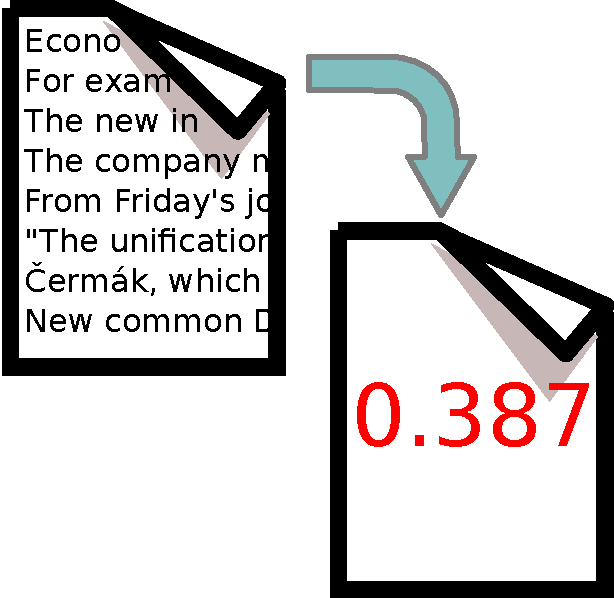
\includegraphics[width=2.5cm]{segment.pdf}
%          \end{center}
%      \end{column}
%  \end{columns}
%  \pause
%  \vspace{1em}
%  \begin{columns}
%      \begin{column}{7cm}
%          \begin{itemize}
%              \item \textbf{Úroveň vět}
%            \begin{itemize}
%              \item Metrika vyprodukovala jedno skóre pro každou přeloženou větu
%              %\item Vypočítal jsem korelaci mezi lidskými párovými porovnánimi a těmi danými metrikou
%            \end{itemize}
%          \end{itemize}
%      \end{column}
%      \begin{column}{3cm}
%          \begin{center}
%            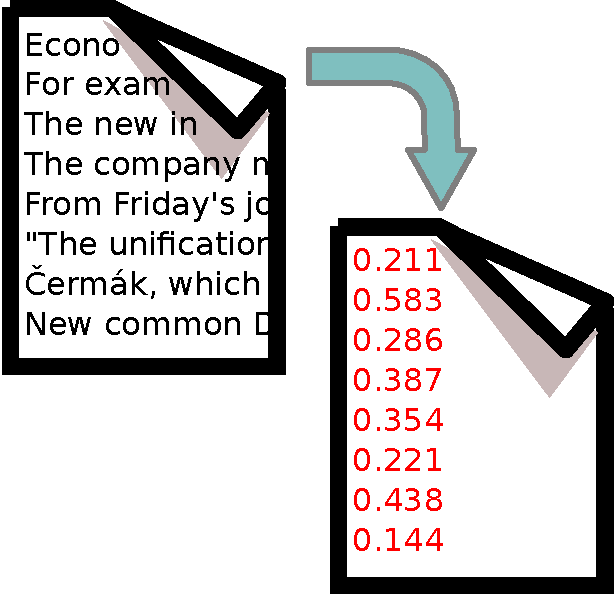
\includegraphics[width=2.5cm]{system.pdf}
%          \end{center}
%      \end{column}
%  \end{columns}
    %\end{frame}

\begin{frame}{Shrnutí soutěže strojových metrik}
    \begin{itemize}
            \pause
        \item 23 metrik z 12 vědeckých týmů, 6 baseline metrik
        \begin{itemize}
            \item Většina z nich je popsána v diplomové práci
        \end{itemize}
            \pause
        \vspace{0.5em}
        \item Představil jsem a v práci diskutuji některé změny, které vedou ke spravedlivější
            evaluaci metrik
        \begin{itemize}
            \item Změnil jsem korelační míru použitou na úrovni systémů
            \item Přestal jsem penalizovat shodné porovnání metrikou
            \item Zavedl jsem počítání konfidenčních intervalů
        \end{itemize}
        \vspace{0.5em}
            \pause

        \item Zveřejnil jsem všechny skripty společně s testovacími daty
        \begin{itemize}
            \item Každý tak může zreprodukovat výsledky nebo vyhodnotit novou metriku
        \end{itemize}
            \pause
        \vspace{0.5em}
        \item Tipy šéfkuchaře pro vývoj nových metrik:
        \begin{itemize}
            \item Používejte rysy z různých lingvistických vrstev
            \item Nezapomeňte ladit parametry své metriky
        \end{itemize}
          \hfill\raisebox{0pt}[0pt][0pt]{
\includegraphics[width=2cm]{chef_says_okay.png}}
    \end{itemize}
\end{frame}

\begin{frame}{Shrnutí}
    \begin{itemize}
        \item Navrhl jsem metodu ručního hodnocení strojového překladu
        \begin{itemize}
            \item Mírně lepší mezianotátorská shoda, pravděpodobně příjemnější pro anotátory
            \item Nelze využít pro hodnocení nových systémů
            \item Mírně pomůže při optimalizaci modelu
        \end{itemize}
                    \pause
            \vspace{0.5em}
        \item Porovnal jsem existující metriky, formou soutěže na WMT
        \begin{itemize}
            \item Úpravy postupu pro spravedlivější porovnání metrik
            \item Veřejně přístupný kód
        \end{itemize}
    \end{itemize}
\end{frame}


%\def\hi#1{\textbf{\textcolor{blue}{#1}}}
%\begin{frame}{System-Level Correlations into English}
%  \vspace{-0.5em}
%  \begin{center}
%  \footnotesize
%    \begin{tabular}{r|cccccc}
%\textbf{From} & \textbf{fr} & \textbf{de} & \textbf{hi} & \textbf{cs} & \textbf{ru} & \textbf{Avg} \\
%\hline
%
% \metric{DiscoTK-party-tuned} & \rangeA{.98}        & \best{\rangeB{.94}} & \rangeA{.96}        & \rangeA{.97}        & \best{\rangeC{.87}} & \best{\rangeB{.94}}\\
% \metric{LAYERED}             & \rangeA{.97}        & \rangeC{.89}        & \best{\rangeA{.98}} & \rangeB{.94}        & \rangeC{.85}        & \rangeB{.93}      \\
% \metric{DiscoTK-party}       & \rangeA{.97}        & \rangeB{.92}        & \rangeC{.86}        & \rangeA{.98}        & \rangeC{.86}        & \rangeB{.92}       \\
% \metric{UPC-STOUT}           & \rangeA{.97}        & \rangeB{.91}        & \rangeC{.90}        & \rangeB{.95}        & \rangeD{.84}        & \rangeB{.91}       \\
% \metric{VERTa-W}             & \rangeA{.96}        & \rangeC{.87}        & \rangeB{.92}        & \rangeB{.93}        & \rangeD{.85}        & \rangeB{.91}       \\
% \metric{VERTa-EQ}            & \rangeA{.96}        & \rangeC{.85}        & \rangeB{.93}        & \rangeB{.94}        & \rangeD{.84}        & \rangeB{.90}       \\
% \metric{tBLEU}               & \rangeA{.95}        & \rangeD{.83}        & \rangeA{.95}        & \rangeA{.96}        & \rangeD{.80}        & \rangeC{.90}       \\
% \metric{BLEU-NRC}            & \rangeA{.95}        & \rangeD{.82}        & \rangeA{.96}        & \rangeB{.95}        & \rangeE{.79}        & \rangeC{.89}       \\
% \baseline{BLEU}                & \rangeA{.95}        & \rangeD{.83}        & \rangeA{.96}        & \rangeB{.91}        & \rangeE{.79}        & \rangeC{.89}       \\
% \metric{UPC-IPA}             & \rangeA{.97}        & \rangeC{.89}        & \rangeB{.91}        & \rangeD{.82}        & \rangeD{.81}        & \rangeC{.88}       \\
% \baseline{CDER}                & \rangeA{.95}        & \rangeD{.82}        & \rangeD{.83}        & \rangeA{.97}        & \rangeD{.80}        & \rangeC{.87}       \\
% \metric{APAC}                & \rangeA{.96}        & \rangeD{.82}        & \rangeE{.79}        & \rangeA{.98}        & \rangeD{.82}        & \rangeC{.87}       \\
% \metric{REDSys}              & \best{\rangeA{.98}} & \rangeC{.90}        & \rangeF{.68}        & \rangeA{.99}        & \rangeD{.81}        & \rangeC{.87}       \\
% \metric{REDSysSent}          & \rangeA{.98}        & \rangeB{.91}        & \rangeF{.64}        & \best{\rangeA{.99}} & \rangeD{.81}        & \rangeC{.87}       \\
% \baseline{NIST}                & \rangeA{.96}        & \rangeD{.81}        & \rangeE{.78}        & \rangeA{.98}        & \rangeD{.80}        & \rangeC{.87}       \\
% \metric{DiscoTK-light}       & \rangeA{.96}        & \rangeB{.93}        & \rangeF{.56}        & \rangeA{.95}        & \rangeE{.79}        & \rangeD{.84}       \\
% \metric{Meteor}              & \rangeA{.98}        & \rangeB{.93}        & \rangeF{.46}        & \rangeA{.98}        & \rangeD{.81}        & \rangeD{.83}       \\
% %\metric{TER}                 & \rangeA{.95}        & \rangeE{.77}        & \rangeF{.62}        & \rangeA{.98}        & \rangeD{.81}        & \rangeD{.83}      \\
% \baseline{WER}                 & \rangeA{.95}        & \rangeE{.76}        & \rangeF{.61}        & \rangeA{.97}        & \rangeD{.81}        & \rangeD{.82}       \\
% \metric{AMBER}               & \rangeB{.95}        & \rangeB{.91}        & \rangeF{.51}        & \rangeF{.74}        & \rangeE{.80}        & \rangeE{.78}       \\
% %\metric{PER}                 & \rangeB{.95}        & \rangeC{.87}        & \rangeF{.41}        & \rangeC{.88}        & \rangeE{.80}        & \rangeE{.78}      \\
% \metric{ELEXR}               & \rangeA{.97}        & \rangeC{.86}        & \rangeF{.54}        & \rangeB{.94}        & \rangeF{-.40}       & \rangeF{.58}       \\
%% XXX Metriky TER a PER jsou schovany, nevadi?
%
%    \end{tabular}
%  \end{center}
%\end{frame}

\end{document}
